\documentclass[11pt,a4paper]{article}
\usepackage[left=1in ,right=1in, top=1in, bottom=1in, footskip=.25in]{geometry}
\usepackage{setspace}
\usepackage{natbib}
\usepackage{float}
\usepackage{graphicx}
\usepackage[noabbrev]{cleveref}


\begin{document}

\noindent Jamis Bruening \\
MnM4SDS (GEOG 788p) \\
Update 1

\onehalfspace

\section{Summary}

The aim of my project is to get a comprehensive sense of the landscape scale processes that are at play within my forest plot.  I want to be very familiar with the study location, the distribution of trees and species within in, and any environmental gradients that exist within the measured properties of the forest (tree height, diameter, canopy type, etc.).  After a bit of data-munging, my first task was to do some exploratory plotting, both spatial and non-spatially, to uncover the main trends in the data that I will further interrogate spatially using the methods we've learned in this class.  After doing so, I ran some preliminary regression models to see how strong these relationships were, and to get a sense of how strong of a spatial component there was in the data.  I chose to predict a tree's crown class, a term used to describe the position of a tree relative to its neighbors within a forest stand, as a function of its height, diameter, and species.  This was promising, as my initial model explained about 60\% of the variance in crown type. I should note I made an assumption here about my variable types and the model I used.  I know that linear regressions are used to predict continuous variables, yet my response variable isn't exactly continuous.  The canopy type is rated on a scale from 1-7, with each integer representing an increasingly less-dominant crown type.  However, since nothing in ecology is continuous, I chose to keep this variable as is because in a way, is it could be interpreted as continuous, essentially a gradient from super-dominant - entirely suppressed.  This is an important distinction that should be noted in interpreting my results moving forward.

My next steps will be to investigate any spatial patterns in my residuals, and exploring the extent to which various ways of incorporating space into my analysis improves my results.  Additionally, I want to explore the spatial auto-correlation structure within my variables of interest and define a heterogeneity measure for the various 5x5 meter transects within the plot.

\section{Figures and results}

At first glance, this is a rich ecological data set.  Inherent to ecology is the spatial component, seen here in \cref{CanopyDBH_PointPlot}.  There are definite spatial trends in both the species distribution and diameter of the trees, as well as likely interaction effects (most of the largest trees are) Eastern White Pine.  This plot is the motivation for much of the spatial analysis to come later in the project.

%% tree locations, by species and DBH
\begin{figure}[H]
\centering
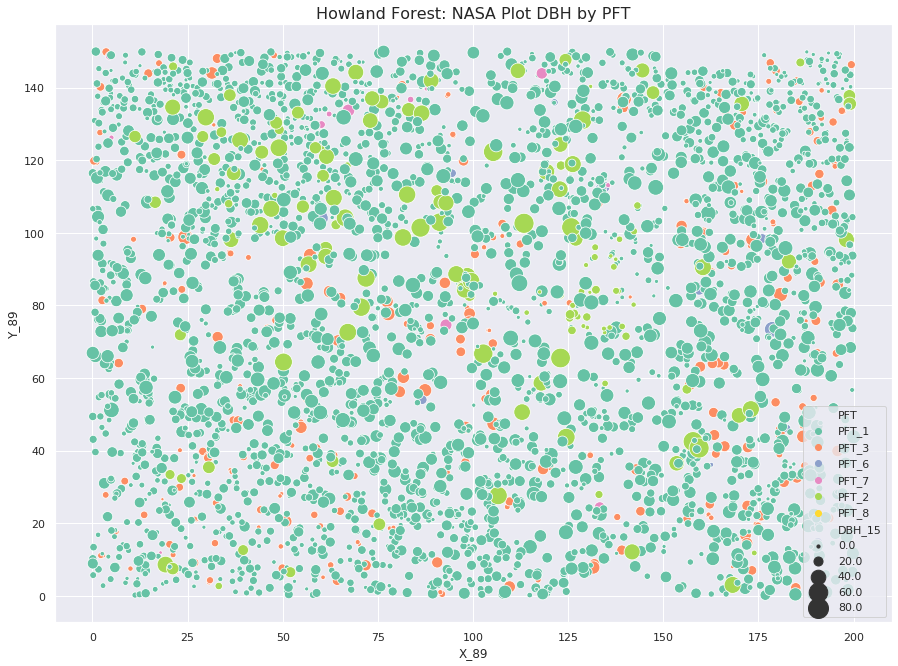
\includegraphics[scale=.5]{../figures/update1/CanopyDBH_PointPlot.png}
\caption{Plot of tree locations, colored by species (SPP), and size based on tree diameter at breast-height (DBH)}
\label{CanopyDBH_PointPlot} 
\end{figure}


My first actual analysis was to predict each tree's canopy class as a function of its height, diameter, and species.  \Cref{Height_and_DBH_by_Canopy_BoxPlot} shows definite relationships between the canopy type and the first two variables, respectively.

%% tree locations, by species and DBH
\begin{figure}[H]
\centering
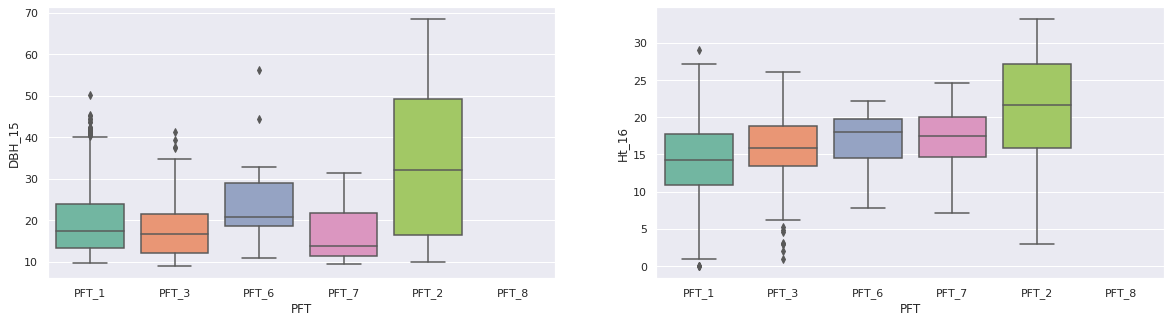
\includegraphics[scale=.4]{../figures/update1/Height_and_DBH_by_Canopy_BoxPlot.png}
\caption{Diameter and height by canopy type}
\label{Height_and_DBH_by_Canopy_BoxPlot} 
\end{figure}

Further, there is also a species effect on the canopy type, seen in \cref{Height_and_DBH_by_Canopy_BoxPlot}.  This is not as pronounced as with height and diameter, but it follows ecological theory that different species of trees may fill different niche spaces in the canopy based on their successional stage and physical properties.  

%% tree locations, by species and DBH
\begin{figure}[H]
\centering
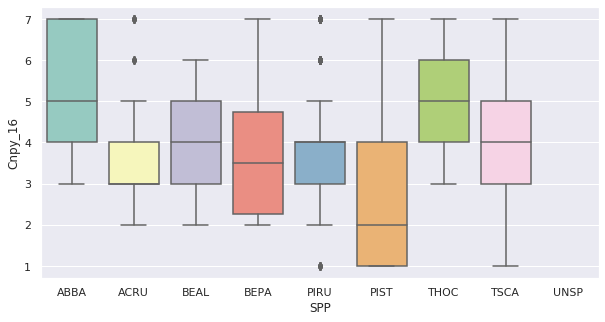
\includegraphics[scale=.4]{../figures/update1/Canopy_by_Species_BoxPlot.png}
\caption{Canopy type by species}
\label{Height_and_DBH_by_Canopy_BoxPlot} 
\end{figure}

Finally, I wanted to quickly assess the colinearity between diameter and height, as these are the most influential predictors of canopy type and are inherently related.  \Cref{Height_DBH_ScatterPlot} shows a definite relationship that is close to linear, yet appears to be slightly logarithmic.  This is what I would expect from ecological theory, as trees are known to continue growing in width after they stop growing in height, due to physical constraints from water limitations.

%% tree locations, by species and DBH
\begin{figure}[H]
\centering
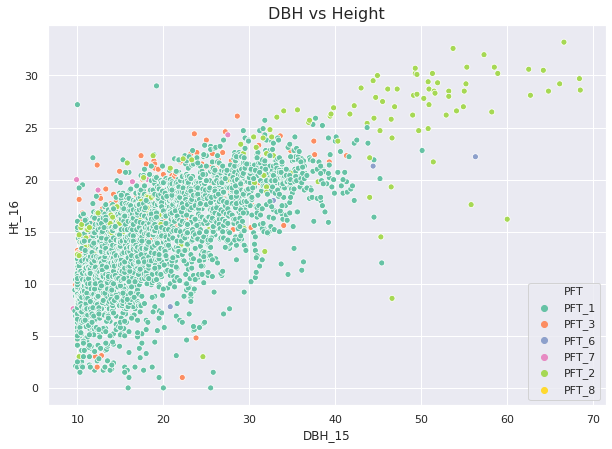
\includegraphics[scale=.5]{../figures/update1/Height_DBH_ScatterPlot.png}
\caption{Tree height as a function of diameter}
\label{Height_DBH_ScatterPlot} 
\end{figure}


% python code to run a logit model (categorical response variable)
%# variables to use in model
%vars16 = ['DBH_15', 'Ht_16']
%# set up variables
%cnpy = np16[['Cnpy_16']].astype(str)
%# run model
%m16 = statsmodels.discrete.discrete_model.MNLogit(cnpy, np16[vars16].values, name_y='Cnpy_16', name_x=vars16)
%m16_fit = m16.fit()
%print(m16_fit.summary())


Putting together the information gained in these plots, I ran a ordinary least squares regression, predicting the canopy type of the tree from these three, relevant variables.  Since the species variable is categorical, I used a fixed effects model to account for this.  This model explains about 60\% of the variance in canopy types, which is relatively good in a ecological context.  However, this being a spatial stats project, I want to further interrogate this data set to identify potential spatial patterns between these variables.

\section{Next steps}

My next steps are to look at the spatial distribution of my model residuals, as well as looking at the spatial autocorrelation of the various environmental variables here.  I'm also interested in looking at the spatial heterogeneity of the 5x5 meter transects, across all three variables.  I can calculate measures of species richness, as well as the mean and standard deviations of height and diameter and see how these vary in space.  This would allow me to turn the points data set into a polygon data set and open up a new set of tools for looking at spatial processes.


%\bibliographystyle{apa}
%\bibliography{proposal.bib}


\end{document}